\section{Evaluation}
\subsection{Testing}
Testing has been accomplished by providing a random\_numbers.py file. With three
separate integer parameters, it creates a random list using Python's standard
random library. The inputs include a lower and upper bound for the list to
generate, together with the length of the list. Once the list is created,
running make will create a .elf file, which contains the parallel mergesort
algorithm with the unsorted list hardcoded within. Once the .elf file is loaded
on a RISC-V processor, it will immediately begin sorting the hardcoded list. The
implementation also needs the value NUM\_CORES defined within the Makefile, where
it both defines a constant NUM\_CORES for the .elf file to use, and the same
value is used for running the QEMU virtual machine.

This gives the following work flow for creating and running a test:
\begin{itemize}
  \item change directory to src/bare\_metal
  \item Run random\_numbers.py to generate alist.c with an unsorted list.
  \item Change the NUM\_CORES variable in the Makefile to the desired number of
    cores.
  \item run "make clean" to remove all files built with previous settings.
  \item run "make test" to generate the .elf file and host qemu. This step will
    create a test.txt file, as the stdout of qemu is redirected to said file.
  \item run "python3 validate.py". This reads the test.txt file, which sorts the
    unsorted array with Python's built in sort function, and compares that sorted
    array with the one produced by the .elf file running in qemu.
\end{itemize}

\subsubsection*{Debugging}
\begin{figure}
  \centering
  \begin{subfigure}[b]{0.45\textwidth}
    \centering
    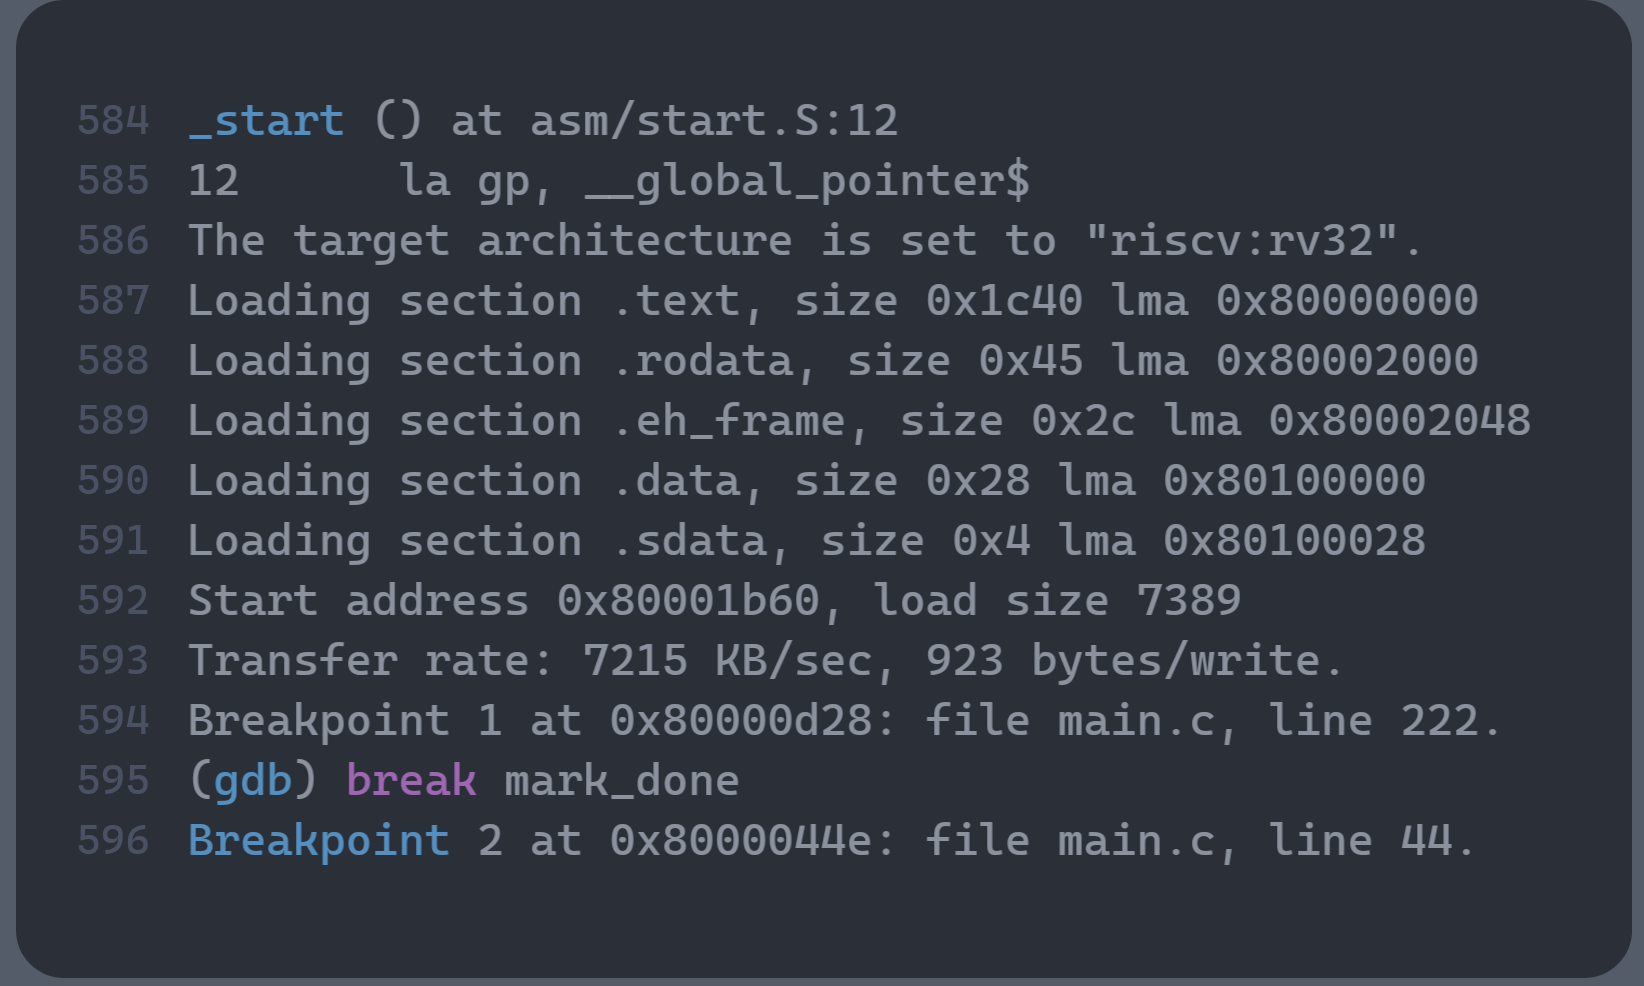
\includegraphics[width=\textwidth]{./figures/debug1.png}
    \caption{Connecting gdb by running "riscv32-unknown-elf-gdb and breaking at
    mark\_done"}
  \end{subfigure}
  \hfill
  \begin{subfigure}[b]{0.45\textwidth}
    \centering
    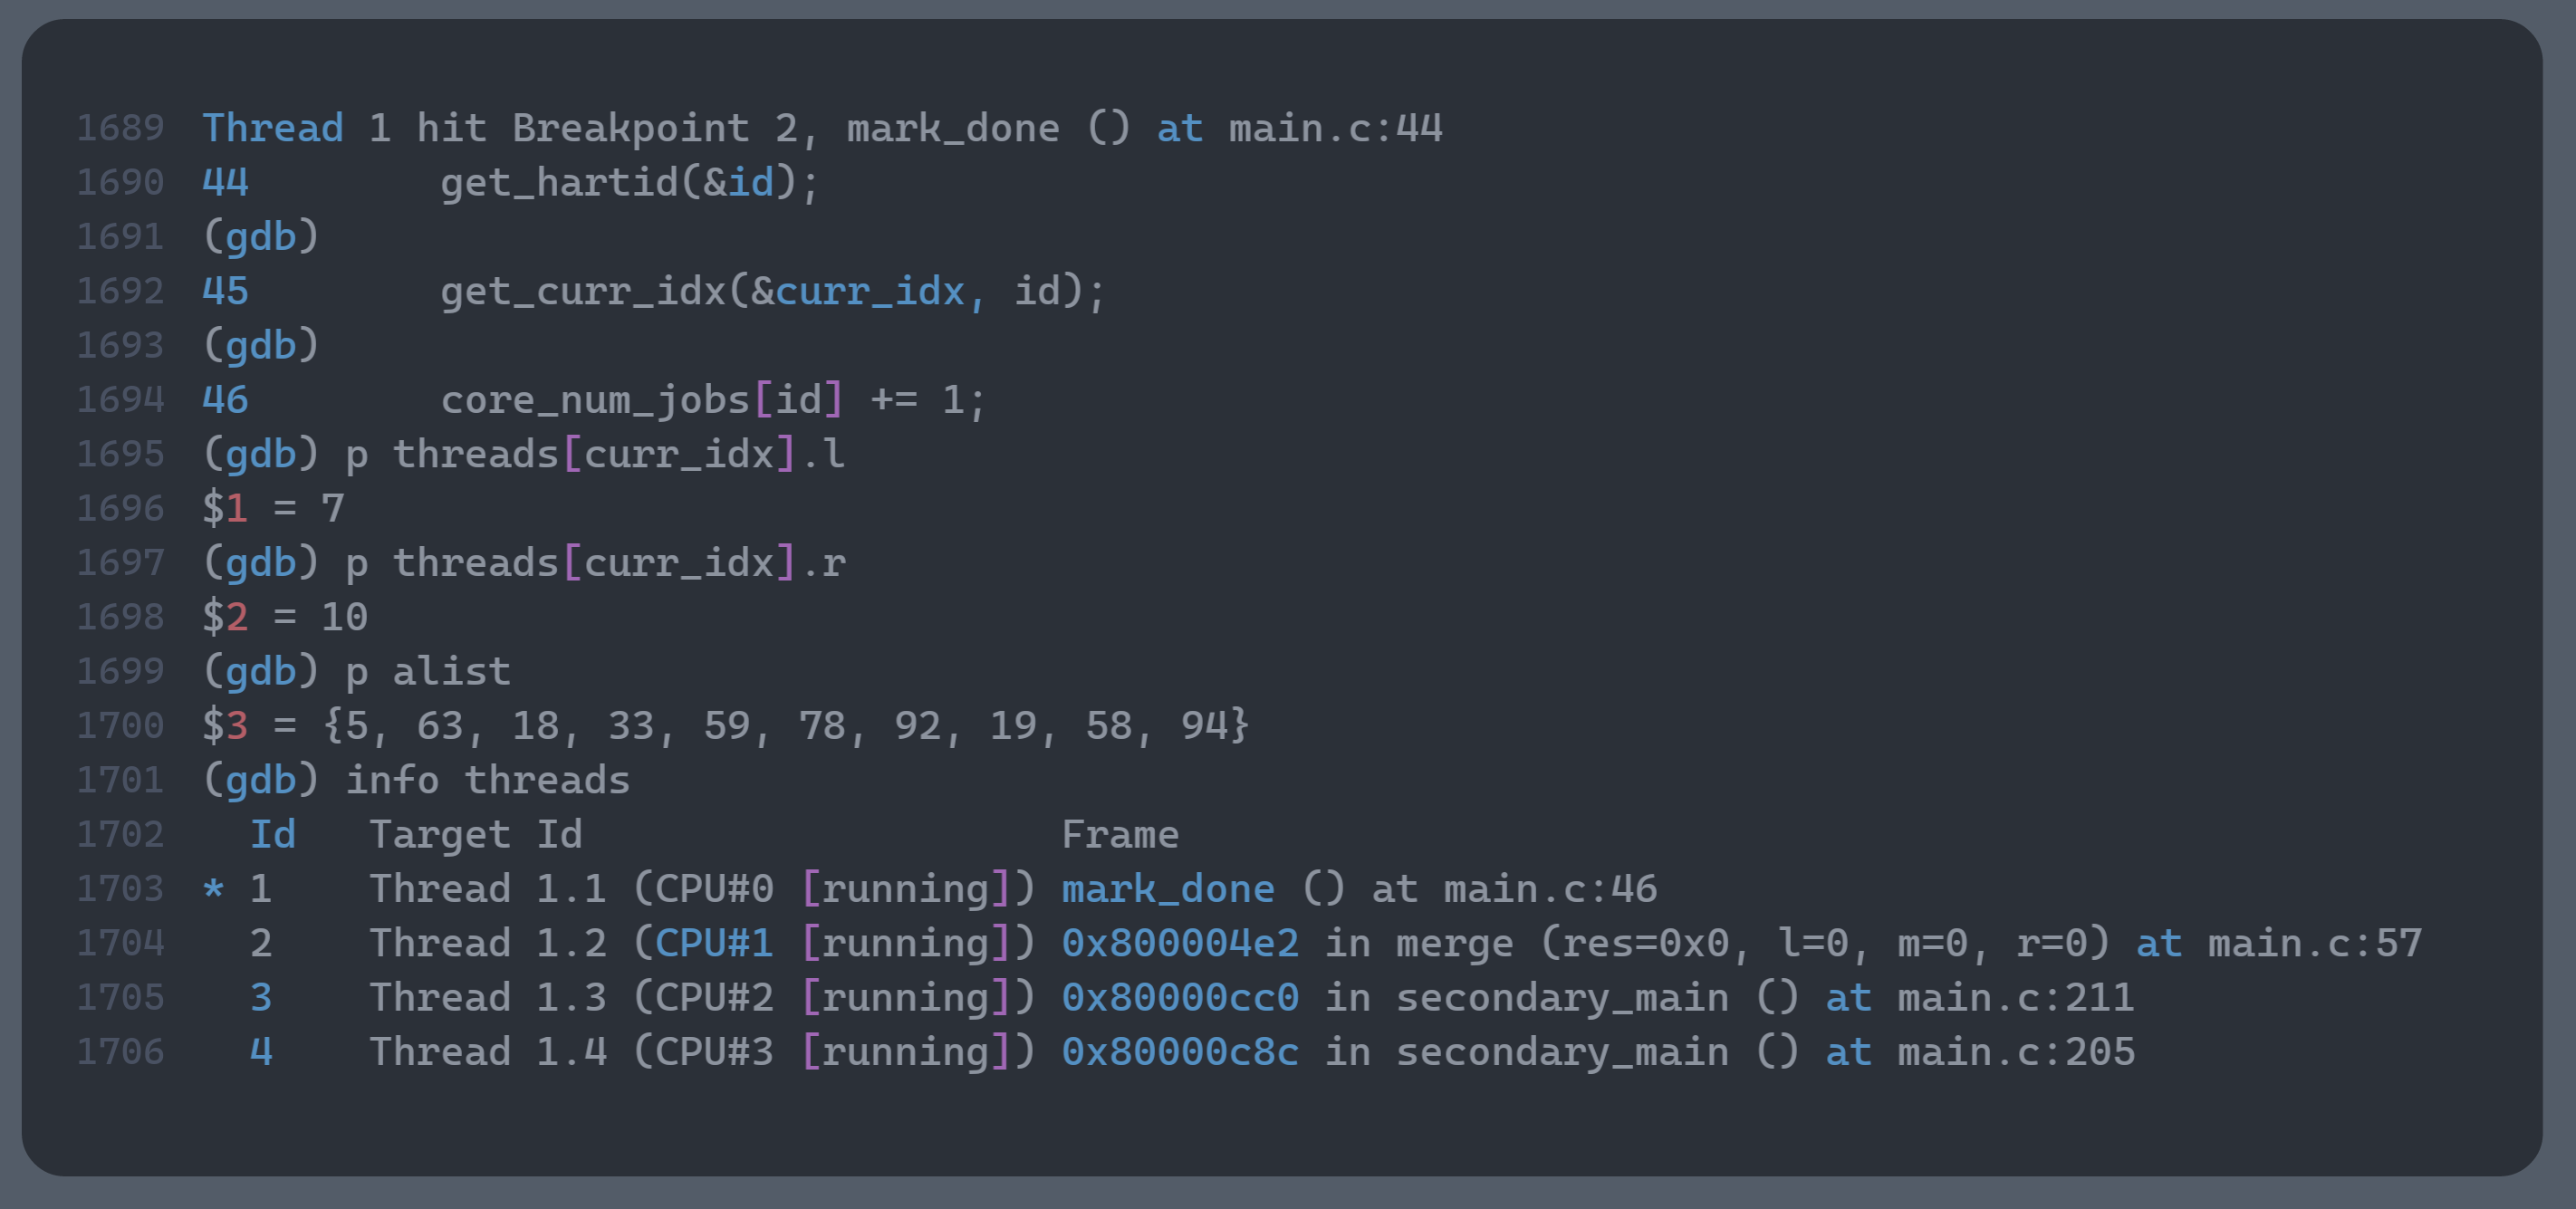
\includegraphics[width=\textwidth]{./figures/debug2.png}
    \caption{Hit breakpoint, where alist is sorted by core 1 from
    index 7 to 10 (10 exclusive).}
  \end{subfigure}
  \caption{Debugging the QEMU virtual machine with 4 cores.}\label{fig:debug}
\end{figure}

To access and debug the multicore system, QEMU provides a way for a remote
gdb-server to connect at the start of execution.\cite{QEMU} In a system where
each core is equivalent gdb will automatically detect the cores, but will
display them as threads. This allows one to debug the QEMU virtual machine with
the same methodology used when debugging multithreaded execution. The workflow shown in Figure~\ref{fig:debug} is as follows:
\begin{itemize}
  \item Change directory to src/bare\_metal.
  \item Initialize the alist.c file with an array and a given size.
  \item Run "make debug" to initialize the QEMU virtual machine.
  \item In a separate terminal instance run "riscv32-unknown-elf-gdb". This will
    automatically run the commands in the ".gdbinit" file and connect to the
    QEMU virtual machine.
  \item Break at mark\_done. This function is run whenever a given thread job is
    finished.
  \item Run "info threads" to get an overview of all threads.
\end{itemize}
As an example Figure~\ref{fig:debug} shows a list of size 10, where core 1 has
sorted the subsection of the list from index 7 to 10. This section corresponds
to one fourth of the list, as the number of cores available is 4.

\subsection{Validation}\label{sec:validate}
\begin{table}
  \caption{Table of tests run}\label{tab:tests}
  \begin{center}
    \begin{tabular}[c]{l|l|l|l|l|l|l}
      & \multicolumn{6}{c}{NUM\_CORES}\\
      \cline{2-7}
      Lower:Upper:Number & 2 & 4 & 8 & 16 & 32 & 64\\
      \hline
      -100:0:100 & pass & pass & pass & pass & pass & pass \\
      \hline
      0:100:100 & pass & pass & pass & pass & pass & pass\\
      \hline
      -50:50:100 & pass & pass & pass & pass & pass & pass \\
      \hline
      -1000:1000:1000 & pass* & pass* & pass* & pass* & pass* & *pass
    \end{tabular} \\
    \vspace{1em}
    \raggedright{\footnotesize *This run initially failed due to stack overflow. After
    increasing the size of STACK\_SIZE to 8192 bytes, THREAD\_STACK\_SIZE to
  8192 and GLOBAL\_STACK\_SIZE 10MB bytes it worked.} \\
  \end{center}
\end{table}

When running a test, the ELF file first prints the unsorted array, and then once
sorting is done, it prints it again. When executing "make test", the QEMU
virtual machine outputs the stdout to a file called test.txt. Subsequently,
invoking python3 validate.py reads this file to ascertain if sorting was
performed correctly. In Table 6, an overview of some tests I conducted can be
seen. On the left, the formatting is specified as the lower bound of randomly
selected numbers, the upper bound, and the number of random elements in the
list. A value of pass signifies that the validate.py file executed without
throwing an assertion error. The tests were initially performed with a global
stack of 0x800,\footnote{defined in ram.ld. Equates to 20,48 bytes.} a
STACK\_SIZE of 2048 and a THREAD\_STACK\_SIZE of 1024. If a failure occurred,
modifications were made to these three values in an attempt to pass the test.

\subsection{Future work}
The implementation proposed in this thesis is more a proof of concept, and as
such comes with a few shortcomings. Firstly, with the current implementation
there is a heavy reliance on the GLOBAL\_STACK\_SIZE. The array to be sorted is
hardcoded and stored on the global stack, which can occupy substantial space
when dealing with large arrays. Furthermore, the array of thread jobs is also
saved on the global stack. with the current implementation each thread type has
a size of 848 bytes. Thus, a solution that reduces overall overall usage of the
global stack, or a better method of detecting the size of the global stack would
allow for a more reliable solution.

Whenever a mergesort splits the into to halves, there is created a new thread
with an allocated stack size of THREAD\_STACK\_SIZE. The top level thread job,
which has to sort the entire array, must first create a copy of the array, before
it can sort in place. The same goes for all other thread jobs, but the amount of
the array they need to copy is halved for each level we move down in the
mergesort tree shown in Figure~\ref{fig:mergesort}. In theory this allows for
halving the size of the allocated thread stack for each level we move down. This
does not take into account the constant space needed for the declared variables,
so the thread stack size might instead be represented by:
\begin{align}
  \text{THREAD\_STACK\_SIZE} = \text{INITIAL\_STACK\_SIZE} / 2^i + C
\end{align}
Where i is the depth level, and C is some constant used to store the variables
needed during computation. This constant C would then be different depending on
whether the given thread has to perform mergesort or just merge over the array.
Experiments determining the size of C could be carried out to optimize the
memory better.

Furthermore, in regards to memory the application does not check whether memory
is out of bounds. Rather, it assumes that the sorting is able to be done with
the allocated memory, and simply lets the application run if there is a stack
overflow on any of the cores or thread stacks. The bounds checking would be
extra overhead, but might still be something worth looking into.

It is not possible for performance testing as the application is running on a
qemu version. Implementing a timing library might be needed to access whether
the performance of multiple cores is significant.
%TODO: this section might need more info.

As it stands the implementation also requires that the number of cores is a
power of 2. This is due to how the initialization builds the threads up. This
issue has a few ways it can be fixed. Firstly, instead of stopping at the same
level for all the merge sorts, it could theoretically split only a few of the
sublist given, such that instead of having to be a power of 2 it would instead
only require that it is a multiple of 2. This would still allow for all cores to
work on a sublist at the same time. Another approach would be to allow a subset
of the number of cores to busy loop until the two child threads as described in
Section~\ref{sec:init_threads}. The former approach seems more promising, but is
left as something which can later be addressed.

As it stands the only method of loading an array onto the processor is by hard
coding the list into the .elf file. Although, this works to show the entire
sorting algorithm, it would not be useful in an actual datacenter unless some
sort of communication protocol is established between the host CPU and the
computational storage device. This communication is left as a problem, that
later has to be solved.




